\documentclass[output=paper]{LSP/langsci} 
\author{Letícia Almeida\affiliation{Laboratoire Dynamique du Langage, UMR 5596, CNRS e Université Lyon 2}\lastand
Cristina Flores\affiliation{Universidade do Minho, CEHUM}
}
\title{Bilinguismo}  
\ChapterDOI{10.5281/zenodo.889439}
\abstract{}
\maketitle
\begin{document}
\section{Introdução} 
\label{sec:almeida_intro}

Os primeiros ensaios sobre o \isi{bilinguismo} definem-no como o domínio perfeito de duas línguas, ou seja, encaram a competência bilingue como um grau idealizado de conhecimento a atingir em ambas as línguas (veja, por exemplo, \citealt{bloomfield1933}). Mais recentemente, a definição de bilinguismo deixou de tomar por base essa noção de proficiência idealizada. O termo `bilingue' passou a designar falantes que possuem competência linguística em pelo menos duas línguas. Essa competência pode ser adquirida de diversas formas, em diferentes idades e contextos e atingir níveis de proficiência variáveis, mas, em todo o caso, é sempre necessário que o falante tenha contacto regular com duas (ou mais) línguas durante um determinado período para que o conhecimento linguístico se construa. Este capítulo foca especialmente os casos em que o contacto com as duas línguas se dá de forma precoce, isto é, na infância. Abordaremos, portanto, as particularidades da aquisição da linguagem quando a criança é exposta a mais de uma língua no seu dia a dia.  

Iremos num primeiro momento descrever quais são os contextos mais comuns em que existe situação de bilinguismo simultâneo.\is{bilinguismo!bilinguismo simultâneo} Num segundo momento, abordaremos a questão da vantagem ou desvantagem desta situação. De seguida, iremos focar-nos na representação das duas línguas no cérebro das crianças bilingues, a partir de uma revisão cronológica dos estudos efetuados sobre esta temática. Seguidamente, faremos referência aos principais processos que influenciam o uso que as crianças fazem das suas línguas. Após a descrição do bilinguismo simultâneo\is{bilinguismo!bilinguismo simultâneo} e as questões relacionadas com a aquisição e o uso de duas línguas desde a nascença, é discutida a importância do fator `idade' na aquisição bilingue, especificamente as particularidades do bilinguismo sucessivo \is{bilinguismo!bilinguismo sucessivo}. Por fim, será abordado um tipo particular de \isi{bilinguismo}, que poderá ser simultâneo ou sucessivo: o \isi{bilinguismo} de herança. Para concluir abordaremos alguns dos fatores que influenciam o desenvolvimento bilingue, nomeadamente a ‘exposição linguística’. O capítulo termina com a descrição do fenómeno de perda de competência linguística em situação de \isi{bilinguismo}.  


\section{Bilinguismo simultâneo:\is{bilinguismo!bilinguismo simultâneo} em que contextos?}%1
\label{sec:almeida_bilinguismo_simul}

É geralmente aceite que, quando uma criança é exposta a duas línguas de forma regular desde a nascença, a criança irá adquirir duas línguas maternas (2\isi{L1}). Nestes casos, as duas línguas a que a criança é exposta são consideradas línguas maternas, uma vez que não existe diferença de tempo entre a primeira exposição a cada uma delas. Considera-se que estes são os casos de \textit{Bilingual First Language Acquisition} (BFLA), ou bilinguismo simultâneo\is{bilinguismo!bilinguismo simultâneo}, por oposição aos casos em que uma segunda língua é introduzida ainda durante a infância, sendo estes últimos os casos de \textit{Bilingual Second Language Acquisition} (BSLA), ou bilinguismo sucessivo\is{bilinguismo!bilinguismo sucessivo}. O termo ‘simultâneo’ vem do facto de a primeira exposição às duas línguas ter ocorrido simultaneamente -- por volta do nascimento, ou pouco tempo depois. 

Como já referido, considera-se que uma criança é bilingue simultânea quando está em contacto com duas línguas desde o nascimento. Esta situação ocorre com bastante frequência, por diversas razões e em diferentes contextos. Em primeiro lugar, uma criança pode estar em contacto com duas línguas desde o primeiro ano de vida nos casos em que vive numa comunidade bilingue, que utiliza duas línguas no quotidiano. Isto verifica-se nos países ou regiões que possuem duas línguas oficiais ou em que, mesmo não havendo explicitamente duas línguas oficiais, as duas línguas são partilhadas e utilizadas pela maioria da comunidade. Situações deste tipo verificam-se com o francês\il{francês} e o inglês\il{inglês} na província de Québec no Canadá, ou ainda com o castelhano\il{espanhol} e o catalão\il{catalão} na Catalunha, ou o castelhano\il{espanhol} e o basco no País Basco, em Espanha. Nestes casos, quando as duas línguas são partilhadas pela comunidade, geralmente as duas são maioritárias e possuem o mesmo nível de prestígio. Por outro lado, a criança também pode estar inserida numa comunidade bilingue em que uma das línguas é tida como minoritária: não é língua oficial. Esse é geralmente o caso das comunidades imigrantes com forte representação num dado país, em que existe suporte social para a utilização das duas línguas, mas uma delas é língua de imigração, também chamada \isi{língua de herança} (cf. \ref{sec:almeida_bilinguismo_heranca}). É o caso das crianças expostas ao castelhano\il{espanhol} e ao inglês\il{inglês} nos Estados Unidos, ou de crianças pertencentes à comunidade portuguesa em França e na Alemanha, ou à comunidade cabo-verdiana em Portugal. Nestes casos, a língua minoritária, de imigração, à diferença dos casos anteriores, é geralmente menos prestigiada do que a língua da comunidade de acolhimento, maioritária. Há ainda casos em que a exposição a duas línguas maternas se dá de maneira quase exclusiva dentro do seio familiar. Esta situação ocorre quando os dois pais possuem línguas maternas diferentes, sendo uma delas a do país de acolhimento, e a outra minoritária. A principal diferença em relação aos casos anteriores é que, geralmente, a língua minoritária não é utilizada por nenhuma comunidade fora de casa, ou é-o por uma comunidade pequena, pouco representada no país de acolhimento. Neste último caso, existe ainda menos suporte social para a utilização da língua minoritária, visto não existir uma comunidade imigrante fortemente representada. A criança acaba por receber muito pouco estímulo da língua minoritária fora de casa; muitas vezes, o estímulo reduz-se praticamente às interações com o cuidador falante dessa língua. Esta última situação é designada de \isi{bilinguismo} familiar, sendo que o único suporte para o \isi{bilinguismo} se encontra no seio da família. No contexto português, inserem-se nesta situação os filhos de casais em que um dos progenitores é falante nativo de uma língua que tem pouca representação como língua de imigração em Portugal, por exemplo o francês,\il{francês} o inglês\il{inglês} ou, ainda, o búlgaro.\il{búlgaro}

As três situações acima descritas constituem os casos mais frequentes de aquisição simultânea de duas línguas maternas \citep{genesee_etal2004} e estão sistematizadas com a ajuda de exemplos no quadro a seguir (Tabela \ref{tab:almeida_1}):

\begin{table}[ht]
\centering
\resizebox{\textwidth}{!}{
\begin{tabular}{llll}
\lsptoprule
                                     &             & Língua maioritária           & País     \\ \midrule
\multicolumn{2}{l}{Língua maioritária (comunidade)} & francês -- inglês            & Canadá   \\ \midrule
\multirow{2}{*}{Língua minoritária}  & comunidade  & português europeu -- francês & França   \\ \cline{2-4}
                                     & familiar    & inglês -- português europeu  & Portugal\\
\lspbottomrule
\end{tabular}}
\caption{Tipos e exemplos de situações de bilinguismo}
\label{tab:almeida_1}
\end{table}

Evidentemente, a fronteira entre uma língua minoritária com suporte na comunidade e uma língua minoritária familiar é ténue e terá de ser estabelecida caso a caso. Esta tipologia é baseada em factos com implicações teóricas mas é possível, por exemplo, que uma criança exposta a uma língua minoritária tipicamente com suporte da comunidade não receba estímulos desse suporte, por ausência de convívio. Tal como é possível que uma língua pouco representada num país seja utilizada de forma consistente por uma pequena comunidade imigrante na qual a criança está inserida. Em todo o caso, é necessário ter em consideração a situação específica de cada criança. 

Embora estes tipos constituam as situações mais frequentes, existem ainda outras possibilidades de uma criança crescer num contexto de \isi{bilinguismo}: a criança pode ser exposta à língua minoritária através de uma ama ou, ainda, a criança pode ter dois pais com línguas minoritárias diferentes para além da língua da comunidade \citep{cruz-ferreira2006}. Neste capítulo, iremos tomar por base os estudos centrados sobre crianças bilingues simultâneas,\is{bilinguismo!bilinguismo simultâneo} independentemente do contexto. Os casos específicos de aquisição do \isi{bilinguismo} no seio de comunidades imigrantes fortemente representadas será abordado de forma mais pormenorizada na Secção \ref{sec:almeida_bilinguismo_heranca}.

Independentemente do contexto de \isi{bilinguismo} acima descrito, o suporte linguístico no seio familiar pode assumir diversas formas. A mais conhecida é o padrão de um pai/uma língua, em que os dois pais possuem línguas maternas diferentes e cada um se dirige à criança na sua língua materna. Esta dinâmica familiar é a mais representada nos estudos sobre bilinguismo simultâneo\is{bilinguismo!bilinguismo simultâneo}, principalmente nos primeiros estudos na área. Por outro lado, os dois pais podem partilhar as duas línguas e dirigirem-se às crianças em ambas, padrão referido como um pai/duas línguas. Noutros casos, um pai pode dirigir-se à criança utilizando duas línguas e o outro apenas uma. Estas diferentes dinâmicas encontram-se esquematizadas e exemplificadas com uma situação de \isi{bilinguismo} português-inglês\il{inglês} na Tabela \ref{tab:almeida_2}:

\begin{table}[h]
\centering
\resizebox{\textwidth}{!}{
\begin{tabular}{llll}
\lsptoprule
           & 1 pai/1 língua & 1 pai/2 línguas    & 1 pai/1 língua e 1 pai/2 línguas \\
\midrule
cuidador 1 & português      & português - inglês\il{inglês} & português                        \\
cuidador 2 & inglês\il{inglês}         & português - inglês & português - inglês\\ 
\lspbottomrule
\end{tabular}}
\caption{Padrões de contacto com as línguas dos pais em situação de bilinguismo}
\label{tab:almeida_2}
\end{table}

A maioria dos trabalhos que se dedicaram ao estudo da aquisição simultânea de duas línguas a partir de meados da década de oitenta consiste em estudos de caso que envolvem o estudo pormenorizado de uma criança exposta a duas línguas através do padrão de `um pai/uma língua'. Apesar de este padrão ter sido o mais estudado na literatura, \citet{dehouwer2009} salienta que é o menos frequente.

A referência a estas situações diversas, quer a nível de dinâmica linguística familiar, quer a nível do suporte social para a utilização das línguas fora de casa, pretende salientar o facto de existir uma grande variedade de situações de \isi{bilinguismo}, o que poderá levar a uma grande variação entre as crianças bilingues simultâneas, quer na utilização das línguas, quer a nível de velocidade de aquisição ou ainda de padrões de desenvolvimento. Para além das propriedades gramaticais de cada língua, que poderão influenciar a aquisição bilingue, é certo que outros fatores também influenciam o \isi{bilinguismo}, tais como a quantidade de exposição que a criança recebe em cada uma das línguas, o prestígio das duas línguas, o incentivo e o suporte social para cada língua, entre muitos outros. No entanto, os estudos conduzidos sobre bilinguismo simultâneo \is{bilinguismo!bilinguismo simultâneo} têm apontado tendências gerais, partilhadas por várias crianças estudadas, que iremos retomar nas próximas secções. 


\section{Bilinguismo infantil: vantagem ou desvantagem?}%2
\label{sec:almeida_bilinguismo_infantil}

Uma das primeiras questões que os investigadores exploraram foi a do impacto da situação de \isi{bilinguismo} no desenvolvimento linguístico e cognitivo da criança. Os primeiros estudos na área do bilinguismo simultâneo\is{bilinguismo!bilinguismo simultâneo} datam do início do século XX. \citet{macnamara1966} propõe uma revisão dos estudos conduzidos até à data, que incidiram na testagem das habilidades linguísticas e cognitivas de crianças bilingues em comparação com crianças monolingues. O autor conclui que, de modo geral, o \isi{bilinguismo} é nefasto para as crianças, pois elas apresentam resultados inferiores às crianças monolingues no que diz respeito não só a habilidades linguísticas como a capacidades de inteligência verbais. O autor estipula ainda que a exposição a duas línguas é prejudicial à criança, no sentido em que ela não só leva mais tempo para adquirir dois sistemas linguísticos, como ainda pode apresentar interferências ou um desenvolvimento mais rápido de um sistema em relação ao outro. Estudos mais recentes refutam este ponto de vista, evidenciando problemas metodológicos nos estudos iniciais: os investigadores raramente tinham em consideração o contexto linguístico das crianças e muitas vezes consideravam o desempenho das crianças bilingues apenas numa das línguas; além disso, comparavam grupos de crianças bilingues e monolingues não homogéneos, havendo variação em muitos outros aspetos, nomeadamente no perfil socioeconómico. Com efeito, estes primeiros estudos compararam crianças bilingues com perfis socioeconómicos inferiores aos das crianças monolingues, pelo que provavelmente seria o estatuto socioeconómico, e não o \isi{bilinguismo}, o fator responsável pela diferença das habilidades encontradas nos dois grupos. Além disso, as crianças bilingues que participaram nesses estudos viviam em contextos em que o \isi{bilinguismo} era desfavorecido: tratava-se de crianças em comunidades de imigração, em que o uso da língua maioritária era incentivado em detrimento da língua minoritária.

Estudos posteriores têm controlado os diferentes aspetos extralinguísticos nas populações de crianças bilingues e monolingues e os resultados têm apontado outras direções. Muitos estudos recentes realçam o efeito positivo do \isi{bilinguismo} em várias tarefas cognitivas \citep{bialystock2001}. Entre várias habilidades cognitivas apontadas como beneficiando do efeito positivo do \isi{bilinguismo}, como a atenção ou a planificação, a que parece apresentar maior disparidade entre crianças bilingues e monolingues é a capacidade de inibição, isto é, a capacidade de ocultar informação na execução de uma tarefa. Um dos testes que permite evidenciar essa capacidade é a arrumação de um jogo de cartas consoante diferentes critérios. Numa tarefa que consiste em pedir às crianças que arrumem um mesmo baralho de cartas por duas vezes, uma vez em função da cor e outra em função do formato, crianças bilingues e monolingues costumam apresentar resultados idênticos aquando da primeira classificação. Contudo, as crianças bilingues acertam mais vezes e mais rapidamente na segunda classificação, ou seja, apresentam uma maior capacidade de ocultar mentalmente a primeira classificação para identificarem a segunda \citep{pearson2009}. É muito provável que esta destreza decorra da capacidade de inibição de um dos seus dois sistemas linguísticos, quando utilizam apenas um. Convém aqui realçar que os efeitos positivos do \isi{bilinguismo} não são sistemáticos: alguns estudos evidenciam um efeito benéfico do \isi{bilinguismo} em tarefas cognitivas, outros evidenciam um efeito negativo e outros, ainda, nenhum efeito. É possível que esses efeitos dependam não só da tarefa como também do nível de proficiência em cada língua \citep{genesee_etal2004}.

Por último, saliente-se que é geralmente evidenciado que as crianças bilingues apresentam melhores níveis de desempenho em tarefas de consciência linguística \citep{genesee_etal2004}. Assim, as crianças bilingues têm mais facilidade em trocar o nome de objetos, percebendo que o objeto designado não se altera por essa razão; por exemplo, percebem mais facilmente que mesmo que a lua se passe a chamar ``sol'', o céu continuará escuro enquanto ela brilhar \citep{pearson2009}. Uma vez que a consciência linguística tem um impacto benéfico na aprendizagem da leitura e da escrita, é esperado que as crianças bilingues também apresentem vantagem durante essa aprendizagem. Esta vantagem tem sido investigada recentemente em estudos conduzidos em grandes grupos de crianças, algumas a frequentarem um ensino monolingue e outras a frequentarem um ensino bilingue inglês\il{inglês}-espanhol\il{espanhol} nos Estados-Unidos. Os resultados evidenciam o efeito benéfico da escolarização bilingue: crianças que aprendem a ler e a escrever em duas línguas apresentam capacidades de leitura superiores às crianças escolarizadas numa única língua logo no segundo ano de escolarização \citep{pearson2009}.

Como vimos, tradicionalmente, a aquisição de duas línguas na infância era vista como tendo custos para a criança, não só a nível cognitivo, como em relação à velocidade de aquisição das duas línguas. \citet{macnamara1966} apresenta uma visão bastante pessimista do \isi{bilinguismo}. De facto, é natural pensar-se que adquirir duas línguas é mais difícil do que adquirir uma só. Para além disso, as crianças bilingues sofrem de outra desvantagem aparente, que é o de ter menos exposição a cada uma das duas línguas. Por outras palavras, as crianças bilingues têm uma tarefa aparentemente mais complicada do que as crianças monolingues, que é a de ter de adquirir duas línguas, tendo uma exposição reduzida a cada uma delas. No entanto, tal como apontado por \citet{meisel2004}, a capacidade de o ser humano adquirir línguas não o predispõe a adquirir apenas uma língua. Meisel afirma que a predisposição para a linguagem é multilingue à partida, permitindo às crianças adquirir uma ou mais línguas, em função do contexto linguístico. Contrariamente aos estudos que avaliam as habilidades cognitivas ou metalinguísticas de crianças bilingues em grandes grupos de crianças, os que se focam sobre o desenvolvimento gramatical têm tradicionalmente por base o acompanhamento longitudinal de poucas crianças, consistindo muitas vezes em estudos de caso. Pretende-se assim fornecer uma visão detalhada do desenvolvimento linguístico, comparando-o com dados de crianças monolingues, também eles muitas vezes obtidos de forma longitudinal e espontânea. Estes estudos que comparam o desenvolvimento linguístico em crianças monolingues e bilingues mostram que, globalmente, a linguagem se desenvolve com uma velocidade semelhante nas duas situações. Evidentemente, existe uma grande quantidade de variação entre crianças, provavelmente maior em crianças bilingues, que poderão não desenvolver as duas línguas à mesma velocidade. No entanto, os estádios principais de desenvolvimento são semelhantes nas duas situações. Assim, sendo bilingue ou monolingue, uma criança geralmente começa a balbuciar entre os 6 e os 12 meses; a primeira palavra costuma ser produzida entre os 12 e os 18 meses; durante o terceiro ano de vida a criança começa a juntar palavras para formar frases; por fim, por volta dos 5 anos de idade, uma criança tem a capacidade de contar uma história curta \citep{dehouwer2009}. Existe apenas uma área da linguagem em que as crianças bilingues apresentam um atraso aparente: a aquisição do vocabulário. Geralmente, as crianças bilingues possuem um vocabulário mais reduzido em cada língua em comparação com crianças monolingues. No entanto, estas crianças nem sempre conhecem a tradução de um item lexical nas duas línguas. Na realidade, quando se contabiliza a totalidade dos conceitos disponíveis no léxico bilingue, em ambas as línguas, o tamanho do vocabulário de crianças bilingues é semelhante ao de crianças monolingues \citep{pearson2009}. 

Na próxima secção, não iremos abordar o estudo do \isi{bilinguismo} infantil com base na comparação com crianças monolingues, mas sim focando-nos nas especificidades da aquisição da linguagem em contexto de \isi{bilinguismo}. 

\section{Qual a relação entre os dois sistemas linguísticos?}%3
\label{sec:almeida_relacao}

Uma questão abordada pelos investigadores na área do bilinguismo simultâneo\is{bilinguismo!bilinguismo simultâneo} prende-se com a natureza das representações linguísticas no cérebro das crianças bilingues. Assim, vários autores questionaram se as crianças bilingues desenvolvem desde o início dois sistemas linguísticos separados ou se começam por tratar os dois sistemas linguísticos como um só. Tal como referido na secção anterior, a maioria das investigações centradas no desenvolvimento gramatical são estudos que se debruçam sobre as produções espontâneas de crianças bilingues, numa perspetiva longitudinal. Os resultados de um primeiro estudo, de \citet{volterrataeschner1978}, apontaram para a evidência da existência, num primeiro momento do desenvolvimento linguístico, de um único sistema de representação dos dois sistemas linguísticos aos quais a criança é exposta. Estes autores, com base no estudo longitudinal das produções espontâneas de duas crianças bilingues italiano\il{italiano}-alemão,\il{alemão} propuseram um modelo de representação bilingue em três estádios: num primeiro momento, os dois sistemas linguísticos encontram-se fundidos; a partir do segundo ano de vida, a representação do léxico separa-se mas o sistema gramatical mantém-se unitário; finalmente, a partir dos três anos de idade, os dois sistemas gramaticais são diferenciados e a criança chega à representação completamente separada dos seus dois sistemas linguísticos. Este modelo é conhecido como a hipótese de `um sistema linguístico unitário'. Na Figura \ref{fig:almeida_1}, esquematiza-se esta proposta, segundo a qual uma criança constrói inicialmente um único sistema de representação linguística quando exposta a \textit{input} contendo duas línguas. 

\begin{figure}
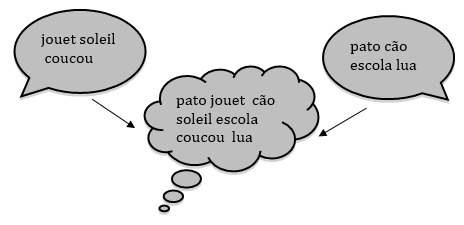
\includegraphics[width=0.95\textwidth]{figures/almeida_1}
\caption{Esquematização da hipótese de um sistema linguístico unitário (adaptação \citealt{genesee_etal2004})}
\label{fig:almeida_1}
\end{figure}

Uma hipótese alternativa é a de ‘dois sistemas linguísticos diferenciados’, proposta por \citet{genesee1989}, \cite{leisel1989} e \cite{dehouwer1990}. Segundo esta visão, as crianças que adquirem duas línguas maternas desenvolvem logo desde o início dois sistemas de representação distintos. Por outras palavras, as crianças constroem desde o início representações separadas para cada uma das línguas a que são expostas, nunca passando por um período de representação unitária. Esta proposta é esquematizada na Figura \ref{fig:almeida_2}:

\begin{figure}
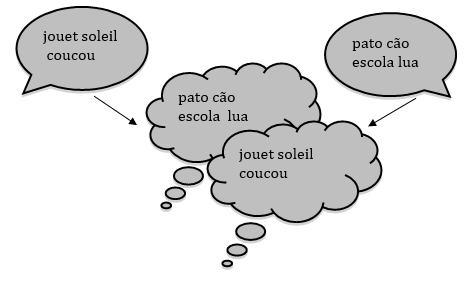
\includegraphics[width=0.95\textwidth]{figures/almeida_2}
\caption{Esquematização da hipótese de dois sistemas linguísticos diferenciados (adaptação de \citealt{genesee_etal2004})}
\label{fig:almeida_2}
\end{figure}

Atualmente, a segunda proposta é a mais aceite pelos investigadores, uma vez que vários estudos têm demonstrado que, em estádios precoces de desenvolvimento, as produções linguísticas das crianças são diferenciadas nas suas duas línguas e que o desenvolvimento linguístico segue padrões diferentes em cada língua, consistentes com as propriedades de cada uma delas. Por exemplo, \cite{cruz-ferreira2003}, com base nas produções espontâneas de três crianças bilingues sueco\il{sueco}-português, com idades compreendidas entre os 0;7 e os 1;9, mostra que as crianças utilizam padrões entoacionais distintos em cada uma das línguas, sendo estes correspondentes aos padrões do adulto. Este estudo, baseado em parte em dados do português, inscreve-se na linha dos resultados de outros estudos dedicados a outras línguas (francês-\il{francês}inglês;\il{inglês} alemão-francês;\il{francês} alemão-italiano,\il{italiano}\il{alemão} entre outras), evidenciando que, em fases precoces do desenvolvimento, as crianças bilingues desenvolvem dois sistemas de representação distintos.

No entanto, o facto de os sistemas serem separados não implica que o seu desenvolvimento seja completamente autónomo. Recentemente, o foco dos estudos sobre bilinguismo simultâneo\is{bilinguismo!bilinguismo simultâneo} alterou-se, tendo-se abandonado a questão da separação das representações iniciais para explorar a questão da independência dos sistemas linguísticos durante a sua aquisição. 

A grande maioria dos estudos dedicados a essa temática tem igualmente por base empírica dados espontâneos longitudinais de poucas crianças avaliadas durante um intervalo considerável de tempo, como por exemplo o estudo de bilingues alemão-francês\il{francês}\il{alemão} \citep{leisel1989} ou holandês-\il{holandês}inglês\il{inglês} \citep{dehouwer1990}. Os resultados desses trabalhos são bastante diversificados. Vários estudos conduzidos no âmbito da sintaxe e da fonologia apontam para um desenvolvimento autónomo das duas línguas enquanto outros apontam para interação entre os dois sistemas \citep{genesee_etal2004,meisel2004}. Assume-se que o desenvolvimento de uma estrutura é autónomo quando os padrões de desenvolvimento em cada língua são distintos e consistentes com as propriedades linguísticas das respetivas línguas-alvo. 

A interação entre os dois sistemas linguísticos pode assumir três formatos: pode existir uma \textbf{\isi{transferência}} de uma estrutura existente numa língua para a outra língua. Pode dar-se o caso de uma dada estrutura se desenvolver de forma mais lenta na criança bilingue em comparação com uma criança monolingue. Neste caso, aponta-se para um \textbf{atraso} no desenvolvimento de uma estrutura. Este caso é provavelmente o mais descrito e atestado na literatura. Enfim, pode acontecer que exista uma \textbf{aceleração} no desenvolvimento de uma estrutura numa língua devido à presença dessa mesma estrutura na outra língua.

Para verificar se existe influência interlinguística entre as duas línguas em aquisição, geralmente comparam-se os padrões de desenvolvimento de crianças bilingues com os de crianças monolingues. Foi com base nesse procedimento que \cite{almeida2011} deu conta de influências interlinguísticas na aquisição fonológica em contexto de bilinguismo simultâneo\is{bilinguismo!bilinguismo simultâneo} (português-francês).\il{francês} Tomemos o exemplo de duas estruturas linguísticas que são adquiridas de forma diferente em crianças monolingues portuguesas e francesas. É o caso dos grupos consonânticos (\underline{fr}uta, \underline{pr}ato, vi\underline{dr}o) e das consoantes em final de sílaba dentro de palavra (fe\underline{s}ta, a\underline{r}te, ba\underline{l}de). Em português, os grupos consonânticos constituem uma estrutura de aquisição tardia, e geralmente as crianças falantes do português europeu produzem uma vogal entre as duas consoantes do grupo numa altura em que ainda não conseguem produzir a estrutura em conformidade com o alvo (cf. \citealt{freitas2017}). Pelo contrário, os meninos franceses costumam adquirir os grupos consonânticos bastante cedo, e sem recorrer à inserção de uma vogal epentética. \cite{almeida2011} notou que a criança bilingue português-francês\il{francês} avaliada exibiu um único padrão na aquisição dos grupos consonânticos em ambas as línguas: foram adquiridos durante o mesmo período de tempo, bastante cedo, sem que a criança recorresse de forma sistemática à inserção de uma vogal epentética. Por outras palavras, a criança exibiu o padrão de desenvolvimento típico do francês\il{francês} na aquisição dos grupos consonânticos em ambas as línguas, indicando uma influência interlinguística durante a aquisição dessa estrutura. Essa influência levou a uma aquisição precoce dos grupos consonânticos em português comparativamente com os monolingues portugueses. 

Na mesma criança, foi observado outro caso de interação linguística que conduziu, desta vez, a um atraso. Tal como nos grupos consonânticos, as crianças monolingues portuguesas e francesas exibem padrões diferentes na aquisição das consoantes em final de sílaba no meio da palavra: as crianças portuguesas exibem uma ordem fixa na aquisição desta estrutura, sendo que a consoante fricativa é adquirida antes das restantes. Este padrão não tem correspondência em francês,\il{francês} visto que geralmente todas as consoantes são adquiridas ao mesmo tempo nessa língua. Uma vez mais, a criança exibiu um padrão único durante a aquisição deste constituinte silábico em ambas as línguas: a criança começou por adquirir as consoantes fricativas, adquirindo as restantes mais tardiamente. Este padrão tem correspondência nos dados das crianças monolingues portuguesas, mas não nos dados das crianças francesas. Desta forma, um novo caso de influência interlinguística é atestado, levando desta vez a um atraso no padrão de aquisição das consoantes em final de sílaba em francês,\il{francês} em comparação com os monolingues franceses.

É importante notar que, nestes dois exemplos, tal como noutros casos descritos para outras línguas, as interações linguísticas ocorrem durante o período de desenvolvimento da linguagem e não interferem no estádio final de aquisição dos sistemas linguísticos: estes acabarão por serem adquiridos e representados em conformidade com o alvo. Assim, as interações são observáveis durante o desenvolvimento linguístico em estruturas específicas e delimitadas. Quando se consideram os padrões gerais de aquisição das duas línguas por crianças bilingues, estes tendem a ser qualitativamente semelhantes aos das crianças monolingues \citep{genesee_etal2004,meisel2004}. Convém realçar que as interações linguísticas fazem parte do desenvolvimento bilingue típico mas têm uma duração limitada no tempo.

Atualmente, ainda não foram totalmente identificados os fatores que poderão determinar a ocorrência de influência interlinguística durante o desenvolvimento simultâneo de duas línguas, nem se essa influência é sistemática ou não. Assim, tem-se apontado para uma grande variação nestes padrões, algumas crianças apresentando influências e outras não. Da mesma forma, o formato das influências também varia bastante entre os estudos, podendo ocorrer atraso, aceleração ou \isi{transferência}. Na realidade, a diversidade de pares de línguas estudados e dos contextos de aquisição, o número reduzido de crianças avaliadas, assim como a variedade das estruturas linguísticas descritas poderão, em parte, explicar estes resultados divergentes. São necessários mais estudos para compreendermos os padrões de autonomia e interação presentes no desenvolvimento bilingue, nomeadamente no que diz respeito aos fatores que os condicionam.


\section{A utilização das línguas pela criança bilingue}%4
\label{sec:almeida_utilizacao}

Na secção anterior, tentámos perceber como são organizadas as línguas num cérebro bilingue. Nesta secção, iremos abordar os comportamentos que as crianças bilingues por vezes apresentam quando utilizam as suas línguas.

Um comportamento frequentemente exibido por uma criança bilingue é o de utilizar preferencialmente uma língua em detrimento da outra, ou até mesmo exprimir-se apenas numa língua. Neste último caso, a criança geralmente entende as duas línguas, mas utiliza apenas uma para se exprimir. Na realidade, é observada uma grande variação na utilização que as crianças bilingues fazem das suas duas línguas. Umas utilizam as duas línguas de modo equivalente, ou pelo menos em função do contexto em que se encontram. Outras têm tendência para escolher espontaneamente sempre a mesma língua, mesmo em contextos em que deveriam utilizar a outra. Nesses casos, as crianças possuem uma língua preferida que utilizam sistematicamente, sendo que apenas recorrem à outra quando o interlocutor dá sinais de não conseguir entender. Em casos extremos pode observar-se um \isi{bilinguismo} passivo, quando as crianças nunca utilizam uma das suas línguas, apesar de terem a capacidade de a entenderem. Muita desta variação decorre de fatores extralinguísticos, como, por exemplo, a quantidade de exposição a cada língua ou o incentivo social para utilizar as duas línguas. É frequente estabelecer-se um perfil de dominância linguística em crianças bilingues com base na sua utilização das línguas, assim como na sua exposição a cada uma delas. De facto, é frequente uma criança preferir ou sentir-se mais à vontade numa das suas línguas. Neste caso, é considerada dominante. Por outro lado, as crianças que utilizam e estão expostas a duas línguas de forma equivalente são consideradas bilingues equilibradas. Evidentemente, esta distinção é muito subjetiva, sendo difícil estabelecer critérios que permitam de facto avaliar a dominância. 

\cite{grosjean2004} afirma que uma propriedade da utilização que os bilingues fazem das suas línguas está relacionada com o conceito de ``modo de língua''. Embora seja aceite que as duas línguas dos bilingues estão ativadas constantemente, o seu grau de ativação varia: por exemplo, perante uma pessoa monolingue, haverá uma menor ativação de uma língua. Por oposição, em situação de fala com outra pessoa bilingue, o bilingue encontra-se num ``modo bilingue'', em que as duas línguas estão praticamente ativadas de igual forma. É neste modo que surgem com frequência os enunciados mistos, isto é, os enunciados que contêm elementos (palavras, morfemas) das duas línguas. Estes enunciados mistos (ou alternância de códigos) constituem um dos argumentos avançados por \cite{volterrataeschner1978} em favor da `Hipótese de um sistema linguístico unitário', como descrito acima. Assim, o facto de as crianças utilizarem num mesmo enunciado elementos pertencentes às duas línguas é interpretado como decorrente da não diferenciação por parte das crianças dos seus dois sistemas linguísticos. No entanto, a alternância de códigos é bastante frequente em adultos bilingues num contexto bilingue; é até a atitude mais natural em vários países multilingues. É com base nesta naturalidade da alternância de códigos entre os adultos que os investigadores afirmam que este comportamento é igualmente um fenómeno natural durante o processo de aquisição da linguagem em contexto de \isi{bilinguismo}. \cite{leisel1989} e \cite{genesee1989} demonstram que a utilização por parte de crianças bilingues de enunciados mistos não constitui evidência de uma confusão ou de uma não diferenciação dos seus dois sistemas. Este comportamento reflete apenas, segundo estes autores, uma estratégia de aquisição das línguas: as crianças bilingues recorrem a todos os recursos que possuem para se exprimirem, sendo que o recurso à outra língua funciona como uma estratégia legítima. Por exemplo, quando as crianças não conhecem uma palavra numa dada língua, têm tendência para utilizar o seu equivalente na outra língua, no caso de o conhecerem. \cite{genesee1989} afirma que os enunciados mistos de crianças bilingues são semelhantes aos dos adultos no sentido em que são regulados gramaticalmente: respeitam as regras gramaticais de ambas as línguas, tais como os dos adultos. Além disso, \cite{genesee_etal2004} salientam que a utilização de enunciados mistos que respeitam as regras gramaticais de cada língua só é possível em bilingues com uma grande proficiência. Portanto, quando as crianças alternam os códigos respeitando a gramática de ambas as línguas, estão a mostrar um comportamento semelhante ao dos adultos, por um lado, e elevada competência em ambas as línguas, por outro lado. Pode haver várias razões que levam as crianças a praticarem a alternância de códigos. Esta pode ocorrer por razões sociais: quando os adultos à volta da criança têm tendência para utilizarem enunciados mistos, as crianças também têm tendência para o fazer com frequência; os enunciados mistos também podem decorrer de fatores pragmáticos ou ainda de uma falha lexical. Apresentam-se de seguida alguns exemplos de enunciados mistos produzidos por uma criança bilingue português-francês,\il{francês} que ilustram a sua utilização no preenchimento de falhas lexicais:

\ea\label{ex:almeida_1}
Exemplos de enunciados mistos de uma criança bilingue português-francês:\il{francês}
 \ea{
\begin{tabbing}
 algumas palavras blablabla \quad \= algumas palavras blablabla \enskip \= falante, xx mses \enskip \= phonet \kill
  \textit{un} peixe \> `um peixe' \> (20 meses)
  \end{tabbing}
}
\ex{
\begin{tabbing}
 algumas palavras blablabla \quad \= algumas palavras blablabla \enskip \= falante, xx mses \enskip \= phonet \kill
  \textit{c'est un} coelhinho \> `é um coelhinho' \> (2 anos)
  \end{tabbing}
}
\ex{
\begin{tabbing}
 algumas palavras blablabla \quad \= algumas palavras blablabla \enskip \= falante, xx mses \enskip \= phonet \kill
  \textit{moi je veux sauver} bolinhas \> `eu quero salvar o bolinhas' \> (3 anos)
  \end{tabbing}
}
\ex{
\begin{tabbing}
 algumas palavras blablabla \quad \= algumas palavras blablabla \enskip \= falante, xx mses \enskip \= phonet \kill
  \textit{moi je mange} flamengo \> `eu como flamengo' \> (3 anos)
  \end{tabbing}
}
\z
\z

Todos estes enunciados ocorreram em sessões em que a língua utilizada pelo interlocutor era o francês.\il{francês} Nos dois primeiros exemplos, a criança recorre a palavras que ainda não conhece em francês:\il{francês} referindo o nome do animal em português, ela mostra possuir o conceito, apesar de não conhecer a etiqueta em francês.\il{francês} Os dois últimos exemplos ilustram uma falha lexical de outro tipo: a palavra portuguesa utilizada não possui uma tradução no léxico do francês.\il{francês} ``Bolinhas'' faz referência a um peluche da criança, sendo este o seu nome; é portanto utilizado aqui como nome próprio, não tendo equivalente em francês.\il{francês} Assim, cada vez que a criança o refere, utiliza o seu único nome (português). Enfim, no último exemplo, a criança está a referir um tipo de queijo português que não existe em França. Logo, a única maneira de o referir é utilizando a sua designação portuguesa. Estes exemplos evidenciam que a criança não mistura as línguas aleatoriamente. Pelo contrário, os enunciados mistos são pouco frequentes nas suas produções e podem ser explicados por situações bem definidas. 

\section{Bilinguismo sucessivo:\is{bilinguismo!bilinguismo sucessivo} qual a importância do fator \textit{idade}?}%5
\label{sec:almeida_bilinguismo_sucess}

O bilinguismo sucessivo\is{bilinguismo!bilinguismo sucessivo} refere-se ao processo de aquisição consecutiva de duas línguas. O indivíduo já adquiriu ou está a adquirir a sua primeira língua (\isi{L1}) quando é exposto a uma segunda língua (\isi{L2}). Uma questão central é, pois, perceber a partir de que momento se deixa de falar de bilinguismo simultâneo\is{bilinguismo!bilinguismo simultâneo} e se passa a designar um contexto de aquisição como sendo sucessivo. 

É relativamente consensual que uma criança parece ter muito mais facilidade em adquirir uma segunda língua do que um adulto. Um indivíduo que, desde a infância precoce, é exposto no seu dia a dia a uma \isi{L2} irá, com muita probabilidade, atingir um estádio final de aquisição semelhante ou muito próximo ao de um falante nativo nos vários domínios do saber linguístico (desde a pronúncia à sintaxe). Pelo contrário, um sujeito que começa a adquirir uma segunda língua em fase adulta, mesmo que viva durante várias décadas no país onde se fala a \isi{L2}, terá muito mais dificuldades em atingir uma competência nativa nessa língua, sobretudo da sua estrutura sonora. Há várias propostas teóricas para explicar esta diferença entre crianças e adultos, sendo aquela que a atribui a fatores de maturação biológica uma das mais influentes. Partindo da proposta original do psicólogo \cite{lenneberg1967}, um número significativo de autores acredita que a faculdade de aquisição da linguagem está sujeita a constrangimentos biológicos e que a capacidade para adquirirmos inconscientemente saber linguístico diminui com o avançar da idade. Esta limitação biológica é designada de `\isi{período crítico}' \citep{lenneberg1967}. Segundo a `Hipótese do Período Crítico',\is{período crítico} a aquisição da linguagem dá-se dentro de uma faixa etária ideal; consequentemente, o conhecimento linguístico adquirido após esse período não se desenvolve de forma nativa. Uma das razões apontadas para esta limitação é a perda de plasticidade neuronal nas zonas cerebrais responsáveis pela faculdade da linguagem. Vários são os modelos teóricos que assentam na hipótese de existência de um \isi{período crítico} para a aquisição da linguagem, como, por exemplo, a `Hipótese da Diferença Fundamental' (\textit{Fundamental Difference Hypothesis}) de \cite{bley-vroman1990}, que define as diferenças essenciais entre a aquisição precoce e a aquisição tardia de uma língua. 

Um desafio para os investigadores que acreditam no papel central do fator idade no processo de aquisição da linguagem é, pois, delimitar a faixa etária a partir da qual o conhecimento linguístico deixa de ser adquirido de forma semelhante à que ocorre desde a nascença, deixando a língua em aquisição de ser classificada como língua materna para ser considerada língua segunda. Este limite está longe de ser consensual. Para Eric Lenneberg, o \isi{período crítico} findaria por volta da puberdade, mas propostas mais recentes propõem que: (i) as alterações na faculdade de linguagem se dão muito mais cedo; (ii) não existe um único \isi{período crítico} para todos os domínios do saber linguístico, mas vários períodos sensíveis que diferem de acordo com a propriedade ou estrutura em aquisição. Quanto à idade que distingue entre bilinguismo simultâneo\is{bilinguismo!bilinguismo simultâneo} e sucessivo,\is{bilinguismo!bilinguismo sucessivo} \cite{meisel2008}, por exemplo, propõe que várias propriedades morfossintáticas deixam de ser adquiridas de forma nativa se a criança contactar com a língua-alvo apenas a partir dos 4 anos de idade. Um caso de aquisição divergente é observada na utilização de pronomes clíticos do francês\il{francês} por parte de crianças bilingues alemão\il{alemão} e francês,\il{francês} que começam a adquirir o francês\il{francês} a partir dos 4 anos de idade. No domínio da estrutura sonora das línguas (por exemplo, a entoação, ou a produção de segmentos vocálicos e consonânticos), alguns autores propõem que esta fase crítica ainda seja mais precoce. \cite{flege_etal1997}, por exemplo, estudaram falantes bilingues de italiano\il{italiano} e inglês,\il{inglês} que começaram a adquirir o inglês\il{inglês} por volta dos 3 anos de idade. Os autores concluem que, apesar da idade precoce da primeira exposição à \isi{L2}, estes falantes apresentam particularidades segmentais e prosódicas na produção do inglês\il{inglês} que os distingue de falantes expostos à língua inglesa desde a nascença.

Entre as várias questões levantadas pela discussão sobre o efeito do fator \textit{idade} no desenvolvimento linguístico, destaca-se o objetivo de perceber qual é, afinal, a diferença entre a aquisição simultânea e a aquisição sucessiva de duas línguas na infância. Sem fazer uma listagem exaustiva das propostas encontradas na literatura, realçamos as seguintes:

\begin{itemize}
\item \textit{Estádio inicial}. No desenvolvimento de duas \isi{L1} simultâneas (2\isi{L1}), a criança apresenta estádios iniciais iguais nas duas línguas, começando por produzir orações de uma palavra e não dispondo de palavras funcionais. No caso da aquisição de \isi{L2}, em níveis iniciais de aquisição, a criança já produz orações mais longas, que contêm elementos funcionais. 
\item \textit{Percurso de aquisição}. Em contexto de 2\isi{L1}, o percurso de aquisição (isto é, as várias fases que se sucedem) tende a ser semelhante à aquisição das respetivas \isi{L1} em contexto monolingue. No caso da criança que adquire uma \isi{L2} depois da \isi{L1}, o percurso de aquisição apresenta mais variação e não é igual às fases de desenvolvimento observadas na aquisição dessa língua enquanto \isi{L1}.
\item \textit{Ritmo de aquisição}. O ritmo de aquisição de duas \isi{L1}s é mais acelerado do que o ritmo de aquisição de uma \isi{L2}.
\item \textit{Transferência\is{transferência} entre línguas}. No caso da aquisição simultânea de duas línguas, a interação entre as línguas em aquisição é mais reduzida do que no caso da relação entre uma \isi{L1} e uma \isi{L2} e parece ter uma duração mais limitada no tempo (cf. Secção \ref{sec:almeida_relacao}).
\item \textit{Uniformidade}. O processo de aquisição de uma \isi{L2} apresenta maior variação entre sujeitos. As crianças que adquirem uma \isi{L2} em idade mais avançada apresentam mais diferenças entre si quanto ao percurso, ritmo e sucesso de aprendizagem do que as crianças que adquirem duas línguas desde a nascença.
\end{itemize}

Há, no entanto, a ressalvar que crianças 2\isi{L1} e crianças \isi{L2} poderão não apresentar diferenças quanto ao estádio final de aquisição, isto é, bilingues sucessivos poderão apresentar um percurso de aquisição diferente de bilingues simultâneos, mas atingir uma competência final muito semelhante. Em muitos casos, em idade adulta, estes falantes são indistinguíveis de falantes de \isi{L1}, sobretudo quando o momento de aquisição da \isi{L2} corresponde a uma mudança significativa de exposição, isto é, a criança passa a estar intensamente exposta à \isi{L2} e deixa de contactar com a sua \isi{L1}. Este é o caso de crianças que foram adotadas por casais de outra nacionalidade e, a partir do momento da adoção, deixaram de contactar com a sua \isi{L1}, passando a ter apenas exposição à \isi{L2} (ver Secção \ref{sec:almeida_erosao}). É, também, o caso de crianças de origem imigrante (p.ex., lusodescendentes), que, em muitos casos, começam apenas a ter exposição mais frequente à língua maioritária, a sua \isi{L2}, quando entram na (pré-)escola, mas esta passa rapidamente a ser a sua língua dominante. As questões relacionadas com este tipo de aquisição bilingue são discutidas na próxima secção.


\section{Bilinguismo de herança}%6
\label{sec:almeida_bilinguismo_heranca}

O termo `\isi{falante de herança}' (FH) entrou na área de investigação sobre aquisição de línguas vindo do contexto norte-americano e para designar um perfil particular de falante bilingue. Originalmente, o termo, proveniente do inglês\il{inglês} `\textit{heritage speaker}', foi proposto pelo investigador canadiano Jim Cummins (veja, p.ex., \citealt{cummins1989}) para designar crianças originárias de famílias imigrantes, que crescem com exposição à língua de origem dos pais, falada no seio da família, e à língua maioritária da sociedade onde vivem. No contexto norte-americano, a investigação sobre falantes de herança\is{falante de herança} foi impulsionada pelas linguistas Silvina Montrul e Maria Polinsky \citep{montrul2008,polinsky2008}, que estudaram comunidades imigrantes de origem hispânica / russa, respetivamente. Porém, a definição que propõem deste tipo de falante bilingue está longe de ser consensual, levantando um conjunto de questões que de seguida discutiremos sucintamente.

Como mencionado acima, o conceito `\isi{falante de herança}' designa especificamente indivíduos provenientes de famílias imigrantes, que já nasceram no país de emigração ou que emigraram ainda na infância, sendo, portanto, emigrantes de segunda (ou mesmo de terceira) geração. Em regra, as crianças de segunda (ou terceira) geração têm contacto com a língua de origem da família no contexto doméstico, na comunicação diária com pais, avós, tios ou outros imigrantes da mesma origem. Geralmente, o contacto com a língua de origem dá-se desde a nascença e é mais intenso nos primeiros anos de vida, antes de a criança entrar no infantário ou (pré-)escola. O contacto com a língua do país de acolhimento, a língua maioritária, intensifica-se quando a criança ingressa no infantário e/ou, mais tarde, na escola, e começa a estabelecer redes de contactos sociais fora da família. Essencialmente, é de realçar que o \isi{falante de herança} tem, desde muito cedo, exposição a duas línguas no seu dia a dia, desenvolvendo conhecimento nativo de dois sistemas linguísticos. Portanto, o \isi{falante de herança} em nada se distingue das definições de falante bilingue revistas nas secções anteriores. Porquê então a necessidade de introdução de um novo termo para designar um tipo de aquisição linguística já muito estudada?

Em primeiro lugar, o termo `\isi{falante de herança}' implica uma caracterização sociolinguística que os termos `bilingue simultâneo', `bilingue precoce' ou `bilingue sucessivo' não têm, pois refere-se especificamente a falantes que crescem em contexto de migração, inseridos numa comunidade imigrante, geralmente com forte representação no país de acolhimento (p. ex., o turco\il{turco} na Alemanha ou o espanhol\il{espanhol} nos EUA), sendo, por isso, falantes de uma língua minoritária, com menor prestígio social. Em regra, estes falantes são escolarizados na língua maioritária, tendo, por vezes, e dependendo do país de emigração, aulas extracurriculares de \isi{língua de herança}, onde adquirem competências de literacia básicas na língua de origem. Como a criança \isi{falante de herança}, nos primeiros anos de vida, em muitos casos, é mais exposta à língua de origem (sobretudo as crianças de 2ª geração), tendo, por vezes, contacto bastante reduzido com a língua maioritária, há alguma dificuldade em definir se o processo de aquisição das duas línguas é \textit{simultâneo} ou \textit{sucessivo}. Se é sucessivo, o que é claramente o caso das crianças que emigram ainda muito novas, a língua de origem é a sua primeira língua (\isi{L1}) e a língua do país de acolhimento é a segunda língua (\isi{L2}). Porém, esta classificação não espelha a particularidade do domínio linguístico destes falantes, pois a língua maioritária rapidamente se torna a sua língua dominante e a primeira língua passa a língua `mais fraca' (do inglês\il{inglês} \textit{weaker language}). Neste sentido, o termo `\isi{língua de herança}' (LH) designa uma língua adquirida desde a nascença, sobretudo em contexto familiar, mas que não é a língua dominante do falante bilingue. O nível de proficiência atingido na \isi{língua de herança} é muito variável, podendo ir de um grau muito baixo no caso de falantes que compreendem a língua de origem, mas que têm competências de produção muito limitadas (os chamados `falantes incipientes' ou `falantes passivos'), a um grau muito elevado, indistinguível da competência de um falante monolingue. Pelo contrário, apesar de o contacto com a língua maioritária muitas vezes se dar apenas aquando da entrada no infantário ou no ensino (pré-)primário, o \isi{falante de herança} tende a atingir competência muito elevada (i.e. nativa) nesta língua. 

Muitos autores que estudam o desenvolvimento de LH assumem que o \isi{falante de herança} adulto tem, em geral, uma baixa proficiência a nível da sua LH, não atingindo o mesmo nível de proficiência que atinge na língua segunda. Esta observação levou autores como Silvina Montrul e Maria Polinsky a propor o termo `aquisição incompleta' (do inglês\il{inglês} `\textit{incomplete acquisition}', cf. \citealt{montrul2008,polinsky2008}) para designar o processo de aquisição de uma LH, descrevendo-o como deficitário e não-nativo. Esta é, porém, a proposta teórica mais debatida nesta área de investigação (veja, por exemplo, a discussão de \citealt{kupischrothman2016}), uma vez que muitos falantes de herança\is{falante de herança} atingem alta proficiência em ambas as suas línguas e o processo de aquisição da sua LH não pode ser designado de incompleto ou não-nativo. Muitos estudos que descrevem a aquisição de uma LH como sendo incompleta e deficitária analisam falantes bilingues que têm um contacto muito limitado com a sua língua de origem, generalizando as suas conclusões, erradamente, a todos os falantes bilingues provenientes de comunidades imigrantes. Contrariando estas observações (muitas vezes limitadas ao contexto linguístico dos EUA), a investigação sobre falantes de herança\is{falante de herança} do português europeu, residentes na Alemanha, mostra que falantes lusodescendentes de segunda geração apresentam, de facto, proficiência linguística muito elevada a nível da sua LH nos vários domínios do saber linguístico \citep{barbosaflores2001,santosflores2013}. Além disso, o conceito de ‘aquisição incompleta’ não é delimitado com precisão, pois, em muitos estudos, a ocorrência de \isi{transferência} interlinguística é descrita como sendo um processo de aquisição incompleta (como no estudo de \citealt{montrul2008}). Uma vez que a maioria dos estudos centrados na aquisição incompleta de uma \isi{língua de herança} analisa falantes adultos (ao contrário dos estudos que focam a aquisição simultânea descrita na secção \ref{sec:almeida_bilinguismo_simul}), estes deparam-se com o problema adicional de não conseguirem separar aquisição incompleta de erosão linguística (conceito revisto na Secção \ref{sec:almeida_erosao}), pois não conseguem determinar se um falante bilingue adulto não possui determinado conhecimento linguístico porque nunca o adquiriu (completamente) ou porque o adquiriu mas voltou a perdê-lo. 

É relevante realçar que a investigação sobre a aquisição de línguas de herança\is{língua de herança} mostra que o processo de aquisição de duas línguas é influenciado, não só por fatores biológicos relacionados com a idade, mas também pela quantidade e pelo tipo de \textit{input} que o falante bilingue recebe. Os efeitos do tipo e da quantidade de exposição às línguas em aquisição constituem o tema central da próxima secção.


\section{A importância do fator \textit{exposição}}%7
\label{sec:almeida_importancia}

Como vimos, a investigação conduzida nas últimas três décadas sobre a aquisição simultânea de duas línguas, com base na observação longitudinal de um número restrito de crianças, tem mostrado que crianças expostas a duas línguas desde a nascença desenvolvem conhecimento nativo das duas línguas e fazem-no de uma forma muito semelhante a crianças monolingues (ver \ref{sec:almeida_bilinguismo_simul}). Uma vez que crianças bilingues, com exposição regular a ambas as línguas no seu dia a dia, (teoricamente) têm o tempo de exposição linguística dividido por duas línguas, este dado mostra-nos que a mente humana consegue desencadear o processo de aquisição nativa de uma língua com quantitativamente menos exposição. Porém, muitos dos estudos de caso longitudinais terminam o período de observação quando a criança tem por volta de 4 a 5 anos de idade, não descrevendo o desenvolvimento da sua competência após esse período. Além disso, o grau de exposição às línguas em aquisição não é um fator controlado neste tipo de estudos, focados em crianças que têm exposição equilibrada às duas línguas no seu dia a dia (por exemplo através da estratégia `um pai/uma língua', cf. \ref{sec:almeida_bilinguismo_simul}). Sabemos, no entanto, que a aquisição de uma língua não termina por volta dos 5 anos, mas prolonga-se até pelo menos os 10 anos de idade e sabemos, também, que o grau de exposição às línguas em aquisição varia muito de criança para criança. Por este motivo, os estudos longitudinais (por exemplo o de \citealt{leisel1989}) deixaram em aberto algumas questões, como:

\begin{itemize}
\item Existem diferenças entre a aquisição de propriedades que estabilizam cedo no desenvolvimento bilingue e a de propriedades que são adquiridas em idades mais avançadas (por exemplo entre os 6 e os 10 anos de idade)?
\item Existem diferenças no processo de aquisição por crianças bilingues que têm exposição equilibrada a duas línguas no seu dia a dia e por crianças que têm um contacto muito reduzido com uma das suas línguas? Se sim, onde estão as diferenças e qual o limite de quantidade de exposição que marca a diferença?
\end{itemize}

A necessidade de responder a estas questões levou ao desenvolvimento, mais recente, de estudos baseados em metodologias experimentais e com grupos maiores de crianças. Entre os estudos que controlam o fator ‘quantidade de exposição’, destacamos a investigação conduzida por Virgínia Gathercole e colegas sobre a aquisição do galês\il{galês} em contacto com o inglês,\il{inglês} no País de Gales, e de Sharon Unsworth sobre a aquisição do holandês\il{holandês} por crianças bilingues na Holanda.

\cite{gathercolethomas2009}, por exemplo, estudam a competência bilingue de crianças da comunidade bilingue do País de Gales nas suas duas línguas oficiais, o inglês,\il{inglês} a língua maioritária, e o galês,\il{galês} que apesar de ser língua oficial é língua minoritária, falada sobretudo (mas não só) no contexto familiar. As autoras mostram que, independentemente da língua de comunicação em casa (inglês,\il{inglês} galês\il{galês} ou ambas), a nível do inglês,\il{inglês} a língua maioritária, os falantes atingem proficiência linguística semelhante à de crianças inglesas monolingues. No entanto, as competências linguísticas desenvolvidas na língua galesa dependem da quantidade de exposição a esta língua. As crianças provenientes de famílias que apenas falam galês\il{galês} em casa apresentam um processo de aquisição do galês\il{galês} muito mais acelerado do que as crianças provenientes de famílias bilingues, que usam o galês\il{galês} e o inglês\il{inglês} na comunicação familiar. Por usar exclusivamente o galês\il{galês} na comunicação no seio da família, o primeiro grupo de crianças tem uma exposição bastante equilibrada às duas línguas, uma falada mais no seio da família e a outra na escola e em contextos sociais fora da família. Já o grupo de crianças provenientes de famílias que usam o galês\il{galês} e o inglês\il{inglês} em casa tem muito mais exposição à língua inglesa do que à língua galesa. Este último grupo apresenta um processo de aquisição mais lento, sobretudo no que diz respeito a propriedades mais complexas, que estabilizam mais tarde no desenvolvimento do galês\il{galês} (por exemplo a categoria `género'). 

Um dado muito interessante deste estudo tem a ver com o facto de, em estádios de desenvolvimento mais avançados, todas as crianças estudadas, independentemente do seu grau de exposição ao galês,\il{galês} atingirem um estádio final de aquisição muito semelhante, ou seja, as crianças com menos exposição à língua minoritária demoram mais tempo a adquirir determinadas propriedades morfossintáticas, mas acabam por adquiri-las em idades mais avançadas. As autoras justificam esta observação com a hipótese de que a aquisição de determinadas propriedades requer uma quantidade mínima de evidência positiva, designada de `massa crítica de exposição' (\textit{critical mass of input}). De acordo com esta hipótese, uma criança bilingue que tenha um contacto mais limitado com uma das suas línguas demorará mais tempo a juntar a massa crítica de exposição necessária à aquisição de determinadas propriedades dessa língua.

De facto, muitos estudos têm realçado o papel central da quantidade de exposição no processo de aquisição bilingue, sobretudo na aquisição de propriedades que estabilizam tardiamente na aquisição nativa. \cite{barbosaflores2001}, por exemplo, demonstram que crianças lusodescendentes, residentes na Alemanha, levam mais tempo a adquirir os contextos que requerem o posicionamento pré-verbal do pronome clítico (= próclise) em português europeu do que crianças monolingues portuguesas. Enquanto crianças monolingues parecem estabilizar o conhecimento de todos os contextos de próclise por volta dos 8 anos, os falantes de herança\is{falante de herança} analisados neste estudo apenas apresentam conhecimento mais estável desta propriedade a partir dos 11 anos de idade. 

Resultados semelhantes são apresentados por \cite{flores_etal2016}, que analisam a produção do modo verbal em orações completivas do português europeu por parte de crianças e adolescentes bilingues luso-alemães,\il{alemão} com idades compreendidas entre os 7 e os 16 anos de idade, num teste de produção provocada (baseado em \citealt{jesus2014}). Este estudo mostra que o facto de as crianças terem dois pais portugueses de primeira geração, que usam dominantemente o português em casa, ou pais bilingues, que usam tanto o alemão\il{alemão} como o português na comunicação com os filhos, influencia significativamente a aquisição do modo conjuntivo na sua \isi{língua de herança}, o português. As crianças que têm menos exposição ao português em casa começam a usar o modo conjuntivo mais tarde do que as crianças com mais exposição.

Uma dificuldade encontrada neste tipo de investigação prende-se com a forma de quantificar a exposição linguística. Quais são, afinal, os fatores que permitem medir a quantidade de exposição de uma criança bilingue às suas línguas? Um contributo importante para a análise dos efeitos da variável `exposição' é dado pelo trabalho de Sharon Unsworth, que tenta quantificar o grau de exposição à língua através de questionários detalhados a pais e professores, tendo em consideração os seguintes fatores:

\begin{itemize}
\item Indivíduos com os quais a criança intervém durante a semana e durante o fim-de-semana (pais, irmãos, tios, avós, ama, educadora de infância, professora, vizinhos, etc.); 
\item Línguas faladas por esses interlocutores e pela criança nesses contextos de comunicação;
\item Número de horas que a criança passa com os interlocutores identificados;
\item Número de horas passadas no infantário / escola e línguas faladas nesse contexto;
\item Número de horas passadas em atividades extracurriculares como fazer desporto, ver televisão, brincar com amigos, ler e jogar computador e línguas usadas nessas atividades.
\end{itemize}

Seguindo uma fórmula de cálculo apresentada em \cite{unsworth2013}, esta quantificação permite ter uma ideia mais ou menos fiável da proporção de contacto com as duas (ou mais) línguas da criança bilingue. Baseando-se nestes critérios, a autora observa que a proporção de exposição ao holandês\il{holandês} das crianças bilingues de holandês-inglês\il{inglês}\il{holandês} investigadas varia, no grupo de crianças estudadas, entre 8\% a 93\% de contacto com o holandês\il{holandês} por semana. Corroborando conclusões de outros estudos que realçam a importância da quantidade de contacto com a língua, \cite{unsworth2013} mostra que há uma correlação significativa entre a proporção de exposição contabilizada para cada criança e a velocidade de aquisição da categoria \textit{género} em holandês,\il{holandês} uma propriedade que, no desenvolvimento nativo desta língua, estabiliza bastante tarde devido à sua opacidade. Naturalmente, as proporções de exposição indicadas em estudos deste género servem para comparar crianças bilingues quanto ao seu grau de contacto com as línguas mas não podem ser entendidas como medidas exatas de quantificação do contacto com cada língua, uma vez que uma quantificação exata é impossível de alcançar devido à natureza variável do objeto de estudo. É ainda de realçar que vários estudos têm mostrado que a variação no grau e tipo de contacto com uma língua não afeta só o desenvolvimento linguístico de crianças bilingues mas também de crianças monolingues. \cite{hartrisley1995}, por exemplo, mostram que há uma correlação significativa entre o número de horas de comunicação no seio da família e a velocidade de aquisição lexical de crianças monolingues.

O contacto que a criança bilingue tem com as duas línguas não varia, no entanto, apenas em relação à quantidade de exposição, mas também à sua qualidade, isto é, ao tipo de \textit{input} que a criança recebe. Porém, é de realçar que a maioria dos fatores que são apontados como determinantes para a qualidade de exposição linguística não são exclusivos de contextos de aquisição bilingues (os seus efeitos também são estudados na aquisição monolingue). Os fatores mais apontados nesta área de investigação são os seguintes:

\begin{itemize}
\item \textit{Variedade de fontes de contacto}. O input da criança é considerado mais rico se ela contacta com a língua-alvo através de diferentes fontes de exposição, como a televisão, amigos, livros, música, etc.
\item \textit{Variedade de interlocutores adultos}. Um fator que pode determinar a qualidade do input é a presença diária de diferentes interlocutores que falem a língua-alvo. Este fator poderá influenciar sobretudo a aquisição fonética.
\item \textit{Variedade de contextos de comunicação/atividades realizadas numa língua}. Os diferentes contextos de comunicação diária implicam o contacto e uso de diferentes registos linguísticos (registo mais formal vs. registo mais familiar), que está associado ao uso de diferentes variedades linguísticas (variedade coloquial, variedade padrão, etc.). Quanto mais variados os contextos de comunicação numa língua, mais contacto a criança tem com diferentes variedades e registos linguísticos. 
\item \textit{Escolarização / nível de literacia}. Sabendo que a instrução formal ajuda a estabilizar o conhecimento de determinadas propriedades linguísticas e que possibilita o contacto com diferentes fontes de \textit{input} linguístico (por exemplo, diferentes tipos de textos escritos), esta é considerada, por muitos autores, uma variável crucial na caracterização do tipo de exposição linguística.
\item \textit{Presença de falantes não-nativos}. Uma vez que a criança bilingue cresce num contexto em que contacta diariamente com duas línguas, nem sempre o input de uma das línguas é fornecido por falantes nativos dessa língua. O número de falantes não-nativos é considerado mais um fator determinante da qualidade do \textit{input}.
\end{itemize}

Embora muitos dos fatores acima enunciados apresentem variação significativa no caso de crianças monolingues, a sua variação é ainda mais elevada em contextos de aquisição bilingue. Uma criança que cresce com duas línguas, em muitos casos, é apenas escolarizada numa das línguas, tendo somente exposição oral coloquial à outra. Por vezes, a criança tem apenas um interlocutor nativo (pai ou mãe) numa das línguas e/ou tem muito contacto com falantes não-nativos dessa língua. Perceber em que medida estes fatores influenciam o processo de aquisição da criança bilingue constitui, assim, mais um desafio que tem despertado a atenção dos investigadores interessados no \isi{bilinguismo}.

O facto de a \isi{língua de herança} de falantes bilingues de segunda geração ser, muitas vezes, considerada diferente da língua falada por um falante nativo está relacionado com os efeitos destes fatores. Geralmente, os falantes de herança\is{falante de herança} não recebem instrução formal na sua \isi{língua de herança} (ou recebem apenas instrução muito limitada) e usam esta língua em contextos informais de comunicação. Isto significa que estão expostos apenas a registos coloquiais e não têm contacto com fontes formais, orais ou escritas. Consequentemente, não contactam com propriedades da língua que estão mais presentes em registos formais e em textos escritos (por exemplo, o uso da mesóclise ou do pretérito mais-que-perfeito simples no português europeu) e apresentam, no seu discurso, marcas da norma coloquial. A falta de instrução formal também explica o baixo grau de consciência metalinguística atribuído a bilingues de herança (para uma discussão destes fatores no \textit{Português Língua de Herança},\is{língua de herança} veja \citealt{flores2015}.)


\section{Erosão linguística: É possível perder uma língua nativa?}%8
\label{sec:almeida_erosao}

Até este ponto, foram discutidas as várias formas de aquisição bilingue, os fatores que influenciam a aquisição precoce de duas línguas e as suas manifestações. Um fenómeno intrinsecamente ligado ao \isi{bilinguismo} e que, por este motivo, tende a ser incluído na área de investigação da aquisição é a perda de competência linguística que, seguindo \cite{flores2008}, designaremos de `erosão linguística' (do inglês\il{inglês} \textit{language attrition}). Excluindo as razões patológicas de perda da linguagem (devido a traumatismos, tumores, acidentes vasculares cerebrais, Alzheimer ou outras demências, etc.), é sobretudo em situações de \isi{bilinguismo} que o fenómeno de erosão linguística é mais expressivo, pois são muito frequentes os casos em que um falante deixa de falar uma língua adquirida na infância por perder o contacto regular com essa língua. Mas é possível o falante perder o domínio dessa língua quando deixa de a usar? Para responder a esta questão é necessário considerar vários fatores, entre eles, (i) a definição de erosão, (ii) a idade da perda de contacto, (iii) a frequência de contacto com a língua em erosão e (iv) o domínio linguístico investigado.

Comecemos por analisar os contextos suscetíveis de erosão linguística, recorrendo à taxonomia proposta por \cite{vanels1986}, que combina o tipo de língua perdida (\isi{L1} / \isi{L2}) com o meio linguístico em que a língua se perde (meio \isi{L1}: o meio linguístico dominante é o da primeira língua do falante / meio \isi{L2}: o meio linguístico dominante corresponde ao da segunda língua do falante):

\begin{figure}
\begin{forest}
	[Língua (em erosão), no edge
		[Meio linguístico dominante, no edge[Tipo de erosão, no edge]]
		]
\end{forest}
\quad
\begin{forest}
	[\isi{L1}
		[meio \isi{L1}[1]]
		[meio \isi{L2}[2]]
		]
\end{forest}
\quad
\begin{forest}
	[\isi{L2}
		[meio \isi{L1}[3]]
		[meio \isi{L2}[4]]
		]
\end{forest}
\caption{Taxonomia de contextos de erosão linguística (baseado em \citealt[4]{vanels1986})
}\label{fig:almeida_3}
\end{figure}

Os tipos 2 e 3 são os contextos de erosão linguística associados ao fenómeno do \isi{bilinguismo} e, consequentemente, os mais estudados nesta área de investigação. O tipo 2, a erosão da primeira língua (\isi{L1}) no meio \isi{L2}, refere-se tipicamente aos casos em que o indivíduo se muda para um meio linguístico diferente (que não seja o da sua \isi{L1}) e com o tempo apresenta efeitos de erosão de aspetos estruturais da sua primeira língua. O tipo 3 da taxonomia de Van Els refere-se à perda de uma \isi{L2} num meio \isi{L1}. Este é o caso típico de falantes bilingues que adquiriram uma segunda língua na infância depois de terem emigrado, mas que deixam de ter contacto com a \isi{L2} quando voltam ao meio linguístico da sua \isi{L1}, por exemplo por terem voltado ao seu país de origem. 

O que importa realçar é que, nos dois contextos suscetíveis de ocorrência de erosão, há uma mudança no meio linguístico dominante: a frequência de contacto com uma das línguas diminui significativamente (ou mesmo completamente) e o falante passa a ter mais exposição à outra língua. Uma das condições para podermos falar de efeitos de erosão linguística é, portanto, a ocorrência prévia de uma mudança das condições de exposição linguística do falante bilingue.

A segunda condição está relacionada com o tipo de conhecimento que o falante possui no momento da alteração das condições de \textit{input}. De facto, só é possível caracterizar alterações na competência de um falante como decorrendo de um processo de erosão se o falante tiver adquirido a propriedade antes da suposta perda. Conhecimento que não tenha sido adquirido não pode ser perdido.

Sintetizando, erosão refere-se, portanto, a uma alteração do conhecimento linguístico, previamente adquirido por um falante bilingue, por motivos de redução de exposição a uma língua (que pode ser uma \isi{L2} ou uma \isi{L1}). Falta, neste ponto, definir o processo de `alteração de conhecimento'. De facto, o conceito de erosão tem sido usado para caracterizar processos muito diferentes, desde alterações nas intuições de falantes nativos adultos em testes de juízos de gramaticalidade à perda total da capacidade de produzir e compreender uma língua adquirida na infância. Este último caso tem sido descrito em estudos sobre falantes adultos que, na infância, foram adotados por casais de outra nacionalidade e deixaram de falar a sua \isi{L1} após a adoção. \cite{pallier_etal2003}, que estudaram falantes de origem coreana adotados por famílias francesas entre os 3 e os 8 anos de idade, atestam uma perda total da \isi{L1} destes falantes, que em fase adulta não são capazes de distinguir o coreano de outras línguas estrangeiras desconhecidas. Os autores concluem que o conhecimento da \isi{L1} foi apagado da mente dos falantes e substituído pela \isi{L2}. Pelo contrário, estudos de cariz mais psicolinguístico, como o de \cite{paradis2004}, defendem que conhecimento adquirido na infância não `desaparece' da mente de um falante, mas é fortemente inibido e poderá ser reativado após reimersão no contexto da língua inibida. Na verdade, os estudos sobre reativação de línguas perdidas/inibidas não são conclusivos quanto a esta questão, que requer mais investigação. 

Um dado consensual na investigação sobre erosão prende-se com a influência do fator `idade'. De facto, os estudos mostram unanimemente que os efeitos de erosão são muito mais severos se o falante bilingue perder o contacto com uma das suas línguas nativas na infância. Já a perda de contacto com a \isi{L1} em fase adulta, mesmo que o falante fique privado de exposição à sua língua nativa durante várias décadas, não parece ter efeitos significativos sobre a competência bilingue. Quanto à idade crítica para manutenção/perda de competência, muitos estudos mostram que a faixa etária dos 10 aos 12 anos é uma idade crítica para a estabilização de saber linguístico \citep{bylund2009,flores2008}. \cite{flores2008} investigou falantes bilingues de alemão\il{alemão} e português que cresceram em país de expressão alemã,\il{alemão} mas vieram viver para Portugal a certa altura da sua vida. O seu estudo mostra que os falantes que perderam o contacto regular com a língua alemã\il{alemão} antes dessa faixa crítica apresentam altos níveis de erosão (por exemplo, a nível da ordem das palavras na frase), enquanto os falantes que regressaram em idades mais avançadas (durante a adolescência) apresentam uma competência bilingue muito estável, mesmo nos casos de falantes que não contactam com o alemão\il{alemão} há mais de vinte anos. Contudo, este estudo incidiu essencialmente sobre o domínio sintático, que -- a par do domínio fonológico -- parece ser uma das áreas mais resistentes à ocorrência de erosão. Pelo contrário, o léxico é o domínio mais vulnerável, pois é (i) a primeira área a ser afetada por sinais de erosão, (ii) a área em que o grau de perda é mais elevado. 

\section{Sumário e conclusões}%9
\label{sec:almeida_sumario}

A aquisição da linguagem em contexto de \isi{bilinguismo} tem sido alvo de um interesse crescente, muito provavelmente por refletir o contexto de aquisição da linguagem por um grande número de crianças. Os estudos desenvolvidos nessa área permitem aprofundar os nossos conhecimentos acerca do funcionamento do cérebro humano. Um dos principais resultados é o de que o nosso cérebro tem a capacidade de adquirir várias línguas sem quaisquer custos cognitivos para a criança. Por outras palavras, a mente humana está biologicamente predisposta a adquirir mais do que uma língua materna se o falante for regularmente exposto a duas (ou mais) línguas desde muito cedo. Se o contacto regular com as duas (ou mais) línguas se mantiver até à adolescência, o falante desenvolve e mantém uma competência bilingue muito estável. A criança bilingue desenvolve precocemente a capacidade de distinguir as suas línguas e o facto de utilizar as duas num mesmo enunciado não é evidência de confusão dos dois idiomas. Sabemos também que, de maneira geral, o desenvolvimento linguístico de uma criança bilingue é semelhante ao de uma criança monolingue, apesar de existirem processos característicos de uma aquisição bilingue, nomeadamente a eventual interação dos dois sistemas durante o seu desenvolvimento. Contudo, é de realçar que a competência bilingue não corresponde à soma de duas competências monolingues, por isso, o falante bilingue pode apresentar particularidades na sua competência linguística que não encontramos em falantes que crescem apenas com uma língua nativa.

Convém não esquecer que as crianças bilingues constituem uma população bastante heterogénea, o que pode explicar em parte a considerável variação observada em diversos trabalhos. Sendo o \isi{bilinguismo} um fenómeno dinâmico, é provável que, ao crescer, as crianças continuem a apresentar perfis diversificados. Algumas poderão tornar-se adultos bilingues equilibrados, outras poderão vir a perder uma das línguas e outras ainda poderão experienciar uma mudança de dominância linguística. 


{\sloppy
\printbibliography[heading=subbibliography,notkeyword=this]
}
\end{document}